% Responsáveis: P2 (classificação), P3 (BERTimbau), P4 (tópicos), P5 (EI)
\section{Resultados}\label{sec:resultados}

\subsection{Classificação}

\begin{table}[t]\centering\scriptsize
\caption{Classificação: validação cruzada com 5 folds agrupados por par, no conjunto de desenvolvimento. F1-macro média $\pm$ desvio-padrão entre folds; IC95\% por bootstrap (1\,000 reamostragens) sobre as previsões \emph{out-of-fold}; F1 por classe; tempo total da CV.}\label{tab:cv}
\begin{tabular}{lccccr}
\toprule
Configuração & F1-macro & IC95\% & F1$_V$ & F1$_F$ & s \\
\midrule
classe maioritária & 0,333 $\pm$ 0,000 & [0,327; 0,339] & 0,667 & 0,000 & 1 \\
só comprimento & 0,944 $\pm$ 0,005 & [0,938; 0,949] & 0,943 & 0,944 & 1 \\
estilo (20 atributos) & 0,965 $\pm$ 0,003 & [0,960; 0,969] & 0,964 & 0,965 & 1 \\
estilo, só proporções (6) & 0,927 $\pm$ 0,007 & [0,921; 0,934] & 0,927 & 0,928 & 1 \\
palavras + LogReg (completo) & 0,972 $\pm$ 0,005 & [0,968; 0,976] & 0,972 & 0,972 & 50 \\
palavras + SVM (completo) & 0,974 $\pm$ 0,006 & [0,970; 0,979] & 0,974 & 0,975 & 46 \\
palavras + LogReg (normalizado) & 0,940 $\pm$ 0,005 & [0,933; 0,945] & 0,940 & 0,939 & 14 \\
palavras + SVM (normalizado) & 0,943 $\pm$ 0,005 & [0,936; 0,949] & 0,943 & 0,942 & 14 \\
caracteres + SVM (normalizado) & 0,956 $\pm$ 0,007 & [0,950; 0,961] & 0,956 & 0,955 & 49 \\
como acaba o texto (normalizado) & 0,890 $\pm$ 0,007 & [0,882; 0,898] & 0,886 & 0,894 & 2 \\
como acaba o texto (cortado) & 0,395 $\pm$ 0,013 & [0,462; 0,486] & 0,337 & 0,611 & 2 \\
palavras + SVM (cortado) & 0,921 $\pm$ 0,006 & [0,914; 0,928] & 0,921 & 0,920 & 8 \\
caracteres + SVM (cortado) & 0,934 $\pm$ 0,002 & [0,928; 0,940] & 0,934 & 0,933 & 27 \\
BERTimbau congelado (normalizado) & 0,970 $\pm$ 0,006 & [0,966; 0,974] & 0,970 & 0,970 & 4 \\
BERTimbau congelado (completo, 512 tok.) & 0,977 $\pm$ 0,002 & [0,973; 0,981] & 0,977 & 0,977 & 4 \\
BERTimbau congelado (cortado) & 0,945 $\pm$ 0,007 & [0,939; 0,950] & 0,945 & 0,945 & 3 \\
BERTimbau fine-tuned (cortado) & 0,987 $\pm$ 0,002 & [0,984; 0,990] & 0,987 & 0,987 & 713 \\
BERTimbau fine-tuned (normalizado) & 0,993 $\pm$ 0,003 & [0,991; 0,995] & 0,993 & 0,993 & 1489 \\
\bottomrule
\end{tabular}\par\smallskip{\footnotesize ``Completo'': texto original; ``normalizado'': versão do corpus com os dois textos de cada par cortados ao mesmo comprimento.}
\end{table}


A Tabela~\ref{tab:cv} resume a validação cruzada. O resultado central é que \textbf{o comprimento,
sozinho, obtém F1-macro de 0,944}. No texto completo, o melhor modelo (TF-IDF de palavras com SVM,
0,974) ganha apenas três pontos a esta \emph{baseline}. Quando se usa o texto normalizado, o TF-IDF
de palavras desce para 0,943, ao nível do comprimento, enquanto o TF-IDF de caracteres mantém 0,956,
com intervalo de confiança que não se sobrepõe ao da \emph{baseline}. As diferenças entre regressão
logística e SVM são pequenas (até 0,3 pontos) e dentro da incerteza.

O BERTimbau obtém os valores mais altos: 0,970 congelado e 0,993 com \emph{fine-tuning}, ambos no
texto normalizado. Estes números devem ser lidos com o artefacto de truncagem em mente: um modelo
que lê o texto por ordem sabe onde ele acaba, e só o final do texto dá 0,890. Na versão cortada,
onde esse sinal não existe, os modelos clássicos perdem pouco (caracteres: 0,956 para 0,934),
confirmando que o sinal de estilo é real.

Sem os dois atalhos, o BERTimbau congelado desce de 0,970 para 0,945, ao nível dos modelos
clássicos, mas o BERTimbau com \emph{fine-tuning} mantém 0,987 [0,984; 0,990], mais cinco pontos
do que o melhor modelo clássico na mesma versão (0,934). Verificámos ainda se este valor vem de
notícias quase repetidas em folds diferentes, que a divisão por pares não apanha: há 51 documentos
com um vizinho de cosseno $\geq0{,}7$ noutro fold, e retirá-los não altera o F1 (0,987). O ganho do
\emph{fine-tuning} tem um custo: 12 minutos de GPU T4 para os 5 folds e 3,6\,GB de memória,
contra segundos em CPU para os modelos lineares. Uma parte do que o modelo aprende pode ser o estilo
editorial do sítio que produziu a maioria das falsas (Secção~\ref{sec:etica}).

\begin{table}[t]\centering\scriptsize
\caption{Resultados no conjunto de teste (1\,444 docs, usado uma única vez). Matriz de confusão como VN/FP/FN/VP (positivo = falsa).}\label{tab:test}
\begin{tabular}{lccccc}
\toprule
Configuração & F1-macro & IC95\% & F1$_V$ & F1$_F$ & VN/FP/FN/VP \\
\midrule
classe maioritária & 0,333 & [0,322; 0,344] & 0,667 & 0,000 & 722/0/722/0 \\
só comprimento & 0,938 & [0,926; 0,951] & 0,939 & 0,938 & 683/39/50/672 \\
estilo (20 atributos) & 0,961 & [0,951; 0,970] & 0,961 & 0,960 & 697/25/32/690 \\
estilo, só proporções (6) & 0,913 & [0,899; 0,927] & 0,913 & 0,913 & 660/62/63/659 \\
palavras + LogReg (completo) & 0,965 & [0,956; 0,974] & 0,965 & 0,965 & 695/27/23/699 \\
palavras + SVM (completo) & 0,973 & [0,965; 0,981] & 0,973 & 0,973 & 702/20/19/703 \\
palavras + LogReg (normalizado) & 0,927 & [0,914; 0,940] & 0,927 & 0,928 & 663/59/46/676 \\
palavras + SVM (normalizado) & 0,935 & [0,922; 0,947] & 0,935 & 0,935 & 672/50/44/678 \\
caracteres + SVM (normalizado) & 0,953 & [0,941; 0,963] & 0,953 & 0,952 & 695/27/41/681 \\
como acaba o texto (normalizado) & 0,892 & [0,876; 0,907] & 0,888 & 0,896 & 619/103/53/669 \\
como acaba o texto (cortado) & 0,404 & [0,383; 0,426] & 0,151 & 0,657 & 63/659/47/675 \\
palavras + SVM (cortado) & 0,907 & [0,892; 0,922] & 0,906 & 0,907 & 651/71/64/658 \\
caracteres + SVM (cortado) & 0,937 & [0,925; 0,949] & 0,937 & 0,937 & 677/45/46/676 \\
BERTimbau congelado (normalizado) & 0,966 & [0,956; 0,974] & 0,966 & 0,966 & 703/19/30/692 \\
BERTimbau congelado (completo, 512 tok.) & 0,972 & [0,962; 0,980] & 0,972 & 0,971 & 709/13/28/694 \\
BERTimbau congelado (cortado) & 0,940 & [0,928; 0,952] & 0,941 & 0,940 & 684/38/48/674 \\
palavras + SVM (cortado, afinado) & 0,913 & [0,899; 0,928] & 0,913 & 0,913 & 659/63/62/660 \\
caracteres + SVM (cortado, afinado) & 0,939 & [0,927; 0,951] & 0,940 & 0,938 & 686/36/52/670 \\
caracteres + LogReg (cortado, afinado) & 0,934 & [0,921; 0,946] & 0,934 & 0,934 & 673/49/46/676 \\
BERTimbau fine-tuned (cortado) & 0,987 & [0,980; 0,992] & 0,987 & 0,987 & 713/9/10/712 \\
\bottomrule
\end{tabular}
\end{table}

O conjunto de teste foi usado uma única vez, com todas as configurações já fixadas
(Tabela~\ref{tab:test}). Os valores coincidem com os da validação cruzada, dentro da incerteza: só
comprimento 0,938 (CV 0,944), caracteres no texto normalizado 0,953 (0,956), caracteres afinados no
texto cortado 0,939 (0,939), BERTimbau congelado no texto cortado 0,940 (0,945) e BERTimbau afinado
0,987 (0,987). O atalho do final repete-se (0,892 no normalizado, 0,404 no cortado). Não houve,
portanto, sobreajuste ao conjunto de desenvolvimento. O BERTimbau afinado erra 19 de 1\,444 notícias
(9 verdadeiras classificadas como falsas e 10 falsas como verdadeiras), e o seu intervalo de
confiança [0,980; 0,992] não se sobrepõe ao do comprimento [0,926; 0,951] nem ao do melhor modelo
clássico [0,927; 0,951]. O critério de sucesso (ii) da Secção~\ref{sec:intro} é cumprido pelo
BERTimbau afinado, mas não pelos modelos clássicos, cujos intervalos se sobrepõem ao da
\emph{baseline} de comprimento.

\subsection{Ablation do pré-processamento}

\begin{table}[t]\centering\small
\caption{Ablation do pré-processamento: TF-IDF + SVM linear no texto normalizado (F1-macro, CV 5 folds no dev).}\label{tab:ablation}
\begin{tabular}{lcc}
\toprule
Pré-processamento & 1-gramas & 1--2-gramas \\
\midrule
sem normalização & 0,933 $\pm$ 0,005 & 0,944 $\pm$ 0,005 \\
minúsculas & 0,930 $\pm$ 0,003 & 0,943 $\pm$ 0,005 \\
+ sem stopwords & 0,923 $\pm$ 0,004 & 0,931 $\pm$ 0,006 \\
+ stemming RSLP & 0,915 $\pm$ 0,005 & 0,928 $\pm$ 0,009 \\
\bottomrule
\end{tabular}
\end{table}


Cada passo de normalização piora o resultado (Tabela~\ref{tab:ablation}): passar de texto
original com bigramas (0,944) a minúsculas, sem \emph{stopwords} e com \emph{stemming} desce até
0,928. Os bigramas ajudam sempre (1 a 1,5 pontos). Estes resultados contrariam a prática habitual
em classificação temática e são coerentes com a hipótese de que o sinal está no estilo: palavras
como ``pra'', ``nesta'' e ``segundo'' são \emph{stopwords} e são das mais discriminativas.

\subsection{Generalização para temas não vistos}

\begin{table}[t]\centering\scriptsize
\caption{Generalização para temas não vistos (\emph{leave-one-topic-out} no dev): treino sem o tema da coluna e teste nesse tema. F1-macro e IC95\%. Documentos de teste: política 3402, TV/celebr. 1188, sociedade 1008, outros 158.}\label{tab:loto}
\begin{tabular}{lcccc}
\toprule
Modelo & política & TV/celebr. & sociedade & outros \\
\midrule
Estilo (6 proporções) & 0,920 {\tiny[0,91; 0,93]} & 0,936 {\tiny[0,92; 0,95]} & 0,936 {\tiny[0,92; 0,95]} & 0,873 {\tiny[0,82; 0,92]} \\
TF-IDF palavras + SVM & 0,888 {\tiny[0,88; 0,90]} & 0,939 {\tiny[0,93; 0,95]} & 0,912 {\tiny[0,89; 0,93]} & 0,860 {\tiny[0,80; 0,91]} \\
TF-IDF caracteres + SVM & 0,911 {\tiny[0,90; 0,92]} & 0,958 {\tiny[0,95; 0,97]} & 0,945 {\tiny[0,93; 0,96]} & 0,911 {\tiny[0,86; 0,95]} \\
\bottomrule
\end{tabular}
\end{table}


Retirar política do treino é o caso mais exigente (Tabela~\ref{tab:loto}): o TF-IDF de palavras
desce de 0,943 para 0,888, enquanto os caracteres (0,911) e os atributos de estilo (0,920) perdem
menos. Em ``outros'' ($n=42$) os intervalos são largos e as conclusões frágeis.

\subsection{Tópicos}

\begin{figure}[t]\centering
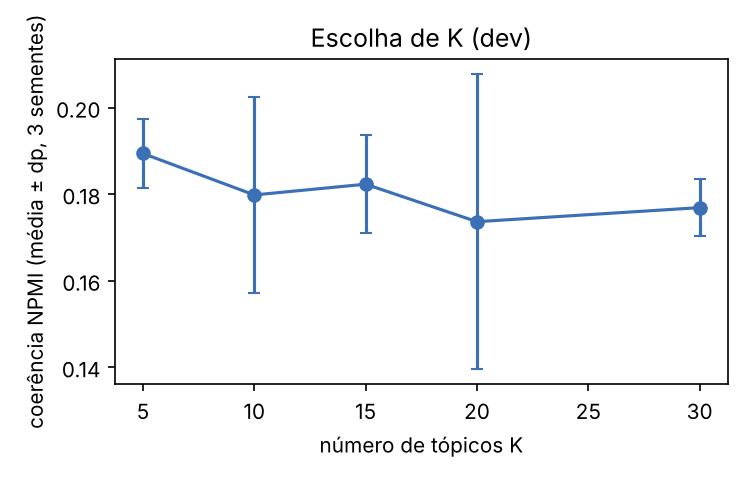
\includegraphics[width=0.42\linewidth]{figs/topicos_coerencia.png}\hfill
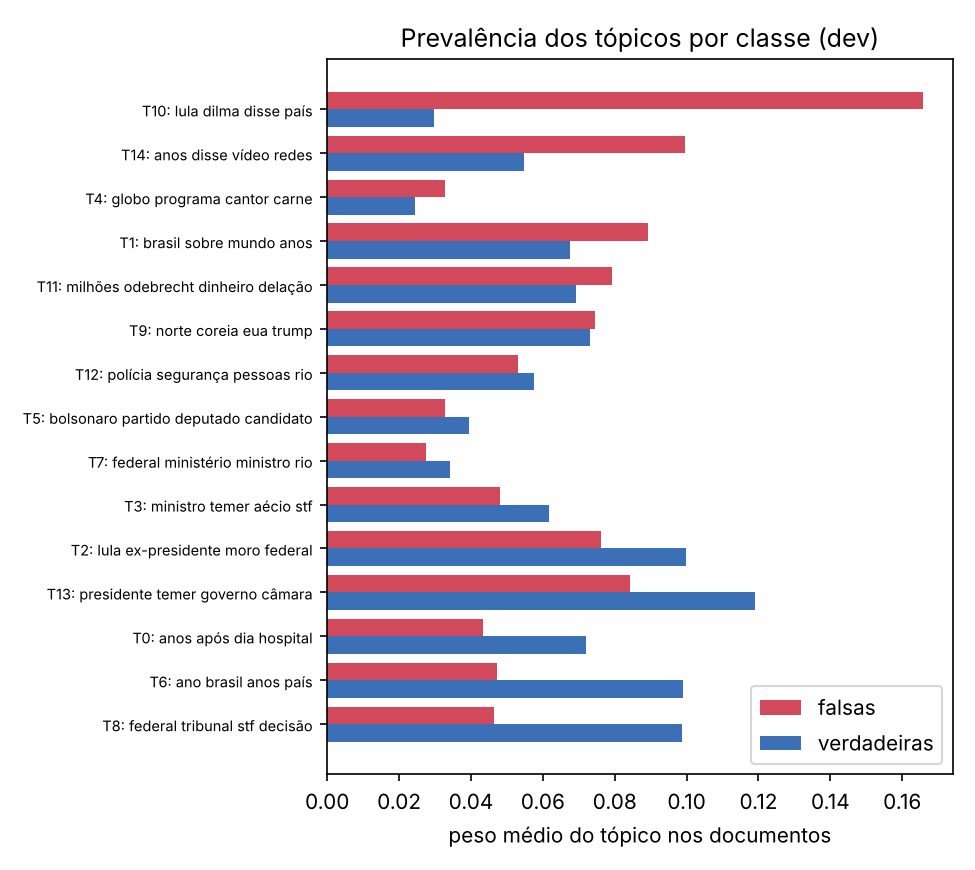
\includegraphics[width=0.55\linewidth]{figs/topicos_por_classe.png}
\caption{Esquerda: coerência NPMI por número de tópicos (média $\pm$ dp de 3 sementes). Direita:
peso médio de cada tópico nas falsas e nas verdadeiras.}\label{fig:topics}
\end{figure}

A coerência quase não varia entre $K=5$ e $K=30$ (Tabela~\ref{tab:k}); as diferenças são da ordem
da variação entre sementes. Escolhemos o maior $K$ cuja coerência fica a menos de um desvio-padrão
da melhor, por analogia com a regra de um erro-padrão~\cite{breiman1984}, o que dá $K=15$ e tópicos
mais finos e interpretáveis. Esta regra foi aplicada depois de observar a curva, o que declaramos
como limitação.

\begin{table}[t]\centering\small
\caption{Escolha do número de tópicos: coerência NPMI média (3 sementes) e perplexidade.}\label{tab:k}
\begin{tabular}{rccc}
\toprule
K & NPMI & dp & Perplexidade \\
\midrule
5 & 0,189 & 0,008 & 3202 \\
10 & 0,180 & 0,023 & 3102 \\
15 & 0,182 & 0,011 & 3133 \\
20 & 0,174 & 0,034 & 3190 \\
30 & 0,177 & 0,007 & 3298 \\
\bottomrule
\end{tabular}
\end{table}

\begin{table}[t]\centering\scriptsize
\caption{Os 15 tópicos LDA (dev), ordenados do mais típico das falsas ao mais típico das verdadeiras.}\label{tab:topics}
\begin{tabular}{lrrrp{4.6cm}}
\toprule
Tóp. & F/V & \%F & Docs & Termos mais prováveis \\
\midrule
T10 Críticas a Lula e ao PT & 5,60 & 93 & 606 & lula dilma disse país vai \\
T14 Histórias familiares e redes sociais & 1,82 & 69 & 454 & anos disse vídeo redes sobre \\
T4 TV Globo e celebridades & 1,35 & 60 & 103 & globo programa cantor carne apresentador \\
T1 Conspirações e temas gerais & 1,32 & 52 & 456 & brasil sobre mundo anos país \\
T11 Delações e corrupção (Odebrecht) & 1,14 & 60 & 443 & milhões odebrecht dinheiro delação empresa \\
T9 Coreia do Norte e EUA & 1,02 & 48 & 432 & norte coreia eua trump kim \\
T12 Polícia e incidentes & 0,92 & 47 & 294 & polícia segurança pessoas rio policiais \\
T5 Eleições de 2018 & 0,83 & 45 & 161 & bolsonaro partido deputado candidato psdb \\
T7 Segurança pública e governo & 0,80 & 42 & 113 & federal ministério ministro rio presos \\
T3 Temer, Aécio e tribunais & 0,78 & 43 & 312 & ministro temer aécio stf senador \\
T2 Lava Jato: Lula e Moro & 0,76 & 43 & 536 & lula ex-presidente moro federal jato \\
T13 Governo Temer e Congresso & 0,71 & 38 & 682 & presidente temer governo câmara michel \\
T0 Acidentes e quotidiano & 0,60 & 34 & 327 & anos após dia hospital ano \\
T6 Saúde e estatísticas & 0,48 & 29 & 419 & ano brasil anos país mil \\
T8 Decisões judiciais & 0,47 & 27 & 418 & federal tribunal stf decisão justiça \\
\bottomrule
\end{tabular}\par\smallskip{\footnotesize NMI(tópico dominante, classe) = 0,047; NMI(tópico dominante, tema) = 0,104. Razão F/V: peso médio do tópico nas falsas a dividir pelo peso nas verdadeiras.}
\end{table}


Dois tópicos concentram as falsas (Tabela~\ref{tab:topics}): \emph{Críticas a Lula e ao PT}
(T10), com peso 5,6 vezes maior nas falsas e 93\% de falsas entre os documentos onde domina, e
\emph{Histórias familiares e redes sociais} (T14). Os documentos mais representativos de T10 têm
marcas opinativas e sensacionalistas (``CRIME!'', ``roubalheira''). Do lado das verdadeiras estão as
\emph{Decisões judiciais} (T8), \emph{Saúde e estatísticas} (T6) e \emph{Acidentes e quotidiano}
(T0). Nem todos os tópicos têm um tema único: \emph{Conspirações e temas gerais} (T1) junta teorias da
conspiração a textos genéricos sobre o Brasil e o mundo. Ainda assim, o tópico dominante está mais
associado ao tema do corpus (NMI 0,104) do que à veracidade (0,047), e uma regressão logística sobre
as 15 proporções de tópicos obtém apenas 0,747 de F1-macro [0,736; 0,758].

\subsection{Extração de informação}

\begin{table}[t]\centering\scriptsize
\caption{Extração de informação: avaliação no ouro anotado manualmente.}\label{tab:ieeval}
\begin{tabular}{llccccr}
\toprule
Correspondência & Tipo & P & R & F1 & IC95\% & $n$ ouro \\
\midrule
estrita & PESSOA & 0,776 & 0,909 & 0,837 & [0,806; 0,865] & 396 \\
estrita & ORGANIZACAO & 0,681 & 0,409 & 0,511 & [0,457; 0,562] & 303 \\
estrita & LOCAL & 0,377 & 0,938 & 0,537 & [0,464; 0,603] & 130 \\
estrita & DATA & 0,716 & 0,765 & 0,739 & [0,650; 0,821] & 102 \\
estrita & TODOS (micro) & 0,634 & 0,735 & 0,681 & [0,653; 0,710] & 931 \\
relaxada & PESSOA & 0,841 & 0,965 & 0,898 & [0,874; 0,920] & 396 \\
relaxada & ORGANIZACAO & 0,725 & 0,429 & 0,539 & [0,485; 0,588] & 303 \\
relaxada & LOCAL & 0,410 & 0,954 & 0,574 & [0,498; 0,639] & 130 \\
relaxada & DATA & 0,881 & 0,922 & 0,901 & [0,852; 0,944] & 102 \\
relaxada & TODOS (micro) & 0,696 & 0,784 & 0,737 & [0,711; 0,762] & 931 \\
\bottomrule
\end{tabular}\par\smallskip{\footnotesize Concordância entre anotadores (F1, 20 docs): 0,875 estrita, 0,931 relaxada.}
\end{table}

\begin{table}[t]\centering\small
\caption{Densidade de entidades por 100 palavras (dev, texto normalizado, \texttt{pt\_core\_news\_md} + regras para datas). Teste de Wilcoxon emparelhado por par ($n=2\,878$).}\label{tab:iedens}
\begin{tabular}{lcccc}
\toprule
Medida & Falsas & Verdadeiras & Mediana F$-$V & $p$ \\
\midrule
Pessoas & 3,99 & 3,33 & 0,48 & $<10^{-4}$ \\
Organizações & 1,42 & 1,57 & 0,00 & 0,0001 \\
Locais & 2,43 & 3,28 & -0,72 & $<10^{-4}$ \\
Datas & 0,43 & 1,28 & -0,73 & $<10^{-4}$ \\
Expressões de atribuição & 0,75 & 0,50 & 0,00 & $<10^{-4}$ \\
\bottomrule
\end{tabular}
\end{table}


No ouro (Tabela~\ref{tab:ieeval}), o extrator tem F1 global de 0,681 (precisão 0,634, revocação
0,735), abaixo da concordância entre anotadores (0,875). As pessoas são o tipo mais fácil (0,837) e as
datas ficam em 0,739. Os locais têm revocação alta (0,938) mas precisão muito baixa (0,377), e as
organizações o inverso (revocação 0,409). A causa é a mesma: o modelo etiqueta instituições como
locais. Das previsões erradas de LOCAL, 103 são organizações no ouro, com destaque para ``STF''
(15 vezes), ``Supremo Tribunal Federal'', ``Congresso'', ``PF'' e ``Ministério Público Federal''.
Ignorando o tipo, o F1 sobe para 0,818: o extrator encontra as entidades, mas erra a sua classe.

Este erro tem consequências na análise. Aplicado a todo o dev (Tabela~\ref{tab:iedens}), o extrator
sugere que as verdadeiras têm mais datas (1,28 vs.\ 0,43 por cem palavras) e mais locais (3,28 vs.\
2,43), e as falsas mais pessoas e mais expressões de atribuição (0,75 vs.\ 0,50). Com a anotação
humana dos 50 pares (Tabela~\ref{tab:iegold}), só a diferença nas \textbf{datas} se confirma, e
até se acentua: 1,24 vs.\ 0,23, cerca de cinco vezes mais nas verdadeiras ($p<10^{-4}$). A
diferença nos locais (1,02 vs.\ 0,69) deixa de ser significativa ($p=0{,}067$): era em grande parte
o efeito de as verdadeiras citarem mais instituições, que o extrator tomava por locais.

\begin{table}[t]\centering\small
\caption{Entidades por 100 palavras segundo a anotação HUMANA (50 pares do dev). Wilcoxon emparelhado por par.}\label{tab:iegold}
\begin{tabular}{lcccc}
\toprule
Tipo & Falsas & Verdadeiras & V/F & $p$ \\
\midrule
Pessoas & 2,82 & 2,48 & 0,9 & 0,124 \\
Organizações & 1,84 & 2,31 & 1,3 & 0,415 \\
Locais & 0,69 & 1,02 & 1,5 & 0,067 \\
Datas & 0,23 & 1,24 & 5,4 & $<10^{-4}$ \\
\bottomrule
\end{tabular}
\end{table}

